\chapter{Los diferentes Steps y sus resultados (StepResult)} \label{sec:steps_detallados}
De manera predeterminada, Samplers provee los Steps que se explican a continuación. Además de los provistos por Samplers, un usuario programador puede definir y agregar sus propios Steps, junto con sus StepFragments y StepResults como se explica en la sección \ref{sec:definir_steps} 

Todos los Step tienen los siguientes campos:

\begin{itemize}
\item \textbf{id:} El identificador del Step, que debe ser único por instancia.
\item \textbf{type:} El tipo de Step, que debe ser uno de los que se detallan a continuación.
\item \textbf{nextStepId:} [Opcional] El identificador del siguiente Step que se debe ejecutar al finalizar con el actual. Si no se especifica, se asume que el Step es el final del Workflow.
\item \textbf{helpFileName:} [Opcional] El nombre del archivo HTML con la ayuda del Step (como se explicó en la sección \ref{sec:mostrar_ayuda}. Si no se especifica, no se mostrará el botón de ayuda para el Step.
\end{itemize}

Además de estos campos, los diferentes tipos de Step agregan campos adicionales como se detalla en la explicación de cada Step a continuación.


\section{PhotoStep: Tomar una foto}
PhotoStep se usa para solicitarle al científico ciudadano que tome una foto. Tiene un texto (text) que se muestran a modo de instrucciones o mensaje cuando la cámara esta encendida. Luego de tomada la foto, se muestra una vista preliminar de la misma, con un botón que da la opción de volver a tomar la foto.

\begin{figure}[H]
  \centering
    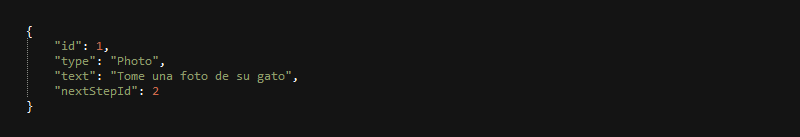
\includegraphics[scale=0.6]{50-anexos/C-steps/photo_json.png} 
    \caption{PhotoStep usando el generador de clases.}
\end{figure}	

\begin{figure}[H]
  \centering
    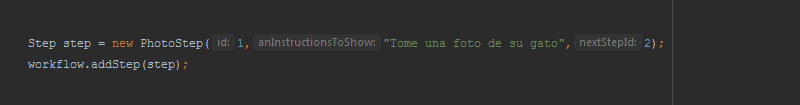
\includegraphics[scale=0.6]{50-anexos/C-steps/photo_java.png} 
    \caption{PhotoStep en Java.}
\end{figure}


\begin{figure}[H]
  \centering
   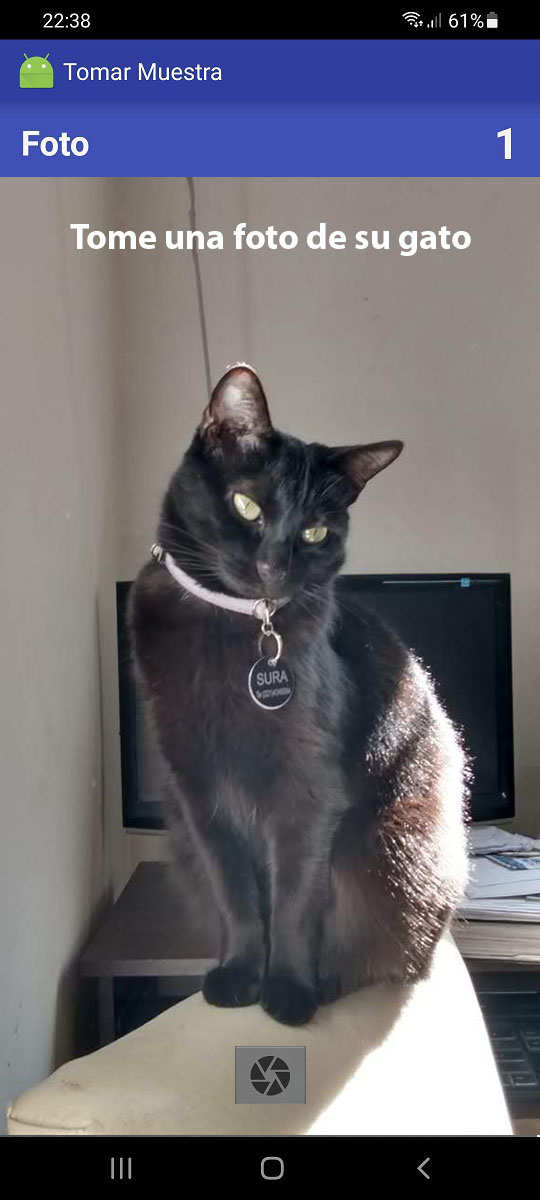
\includegraphics[scale=0.23]{50-anexos/C-steps/photo_screen1.jpg} 
   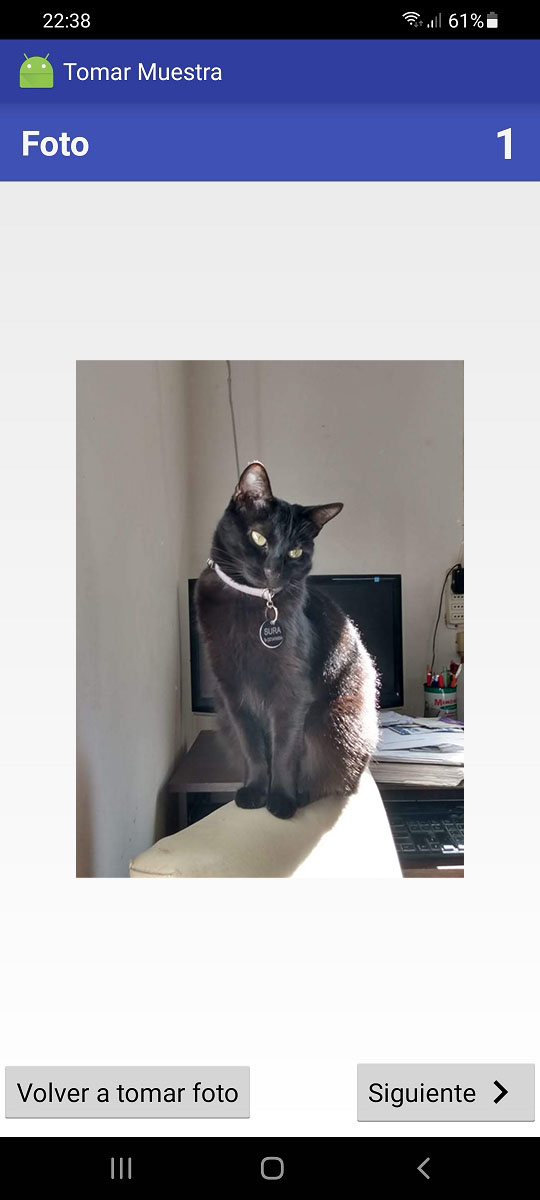
\includegraphics[scale=0.23]{50-anexos/C-steps/photo_screen2.jpg}    
    \caption{Ejemplo de un PhotoStep en ejecución. A la izquierda al momento de tomar la foto, y a la derecha al momento de mostrar la vista preliminar.}
\end{figure}

\subsection{PhotoStepResult: El resultado de Tomar una foto}
El PhotoStepResult contiene el nombre del archivo de la foto tomada. La foto va como archivo jpg en la carpeta de la muestra.
Puede haber varias fotos si hay varios PhotoSteps en el Workflow.




\section{SoundRecordStep: Grabar sonido}
SoundRecordStep  se usa para solicitarle al científico ciudadano que grabe un sonido. Tiene un texto (text) que se muestran a modo de instrucciones o mensaje. Luego de grabado el sonido, el mismo se puede escuchar, y en todo caso volver a grabar otro sonido.


\begin{figure}[H]
  \centering
    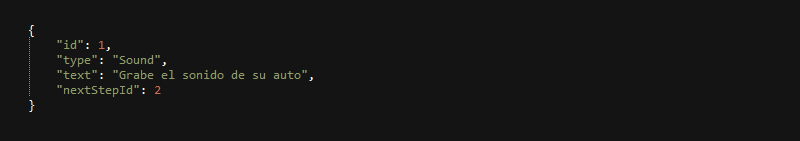
\includegraphics[scale=0.6]{50-anexos/C-steps/sound_json.png} 
    \caption{SoundRecordStep usando el generador de clases.}
\end{figure}	

\begin{figure}[H]
  \centering
    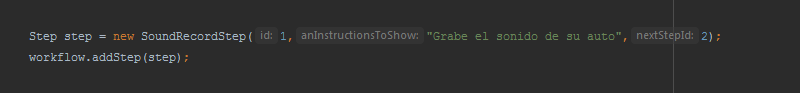
\includegraphics[scale=0.6]{50-anexos/C-steps/sound_java.png} 
    \caption{SoundRecordStep en Java.}
\end{figure}

\begin{figure}[H]
  \centering
    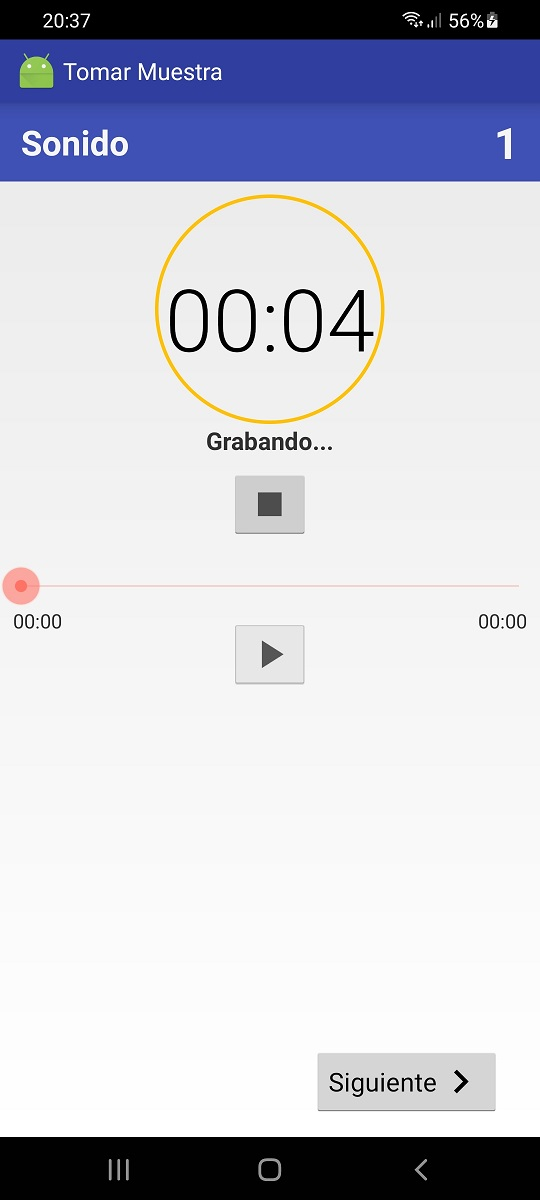
\includegraphics[scale=0.3]{50-anexos/C-steps/sound_screen.jpg} 
    \caption{InsertTextStep en ejecución.}
\end{figure}



\subsection{SoundRecordStepResult: El resultado de Grabar sonido}
El SoundRecordStepResult contiene el nombre del archivo del sonido grabado. El sonido va como archivo mp4 en la carpeta de la muestra.
Puede haber varios sonidos si hay varios SoundRecordSteps en el Workflow.



\section{InformationStep: Mostrar información}
InformationStep se usa para mostrar una información (texto) al científico ciudadano, por ejemplo, para mostrar un mensaje de bienvenida o para explicar brevemente los pasos que seguirán a continuación para tomar la muestra.


\begin{figure}[H]
  \centering
    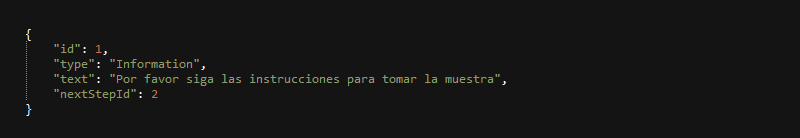
\includegraphics[scale=0.6]{50-anexos/C-steps/information_json.png} 
    \caption{InformationStep usando el generador de clases.}
\end{figure}	

\begin{figure}[H]
  \centering
    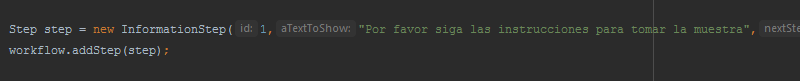
\includegraphics[scale=0.6]{50-anexos/C-steps/information_java.png} 
    \caption{InformationStep en Java.}
\end{figure}


\begin{figure}[H]
  \centering
    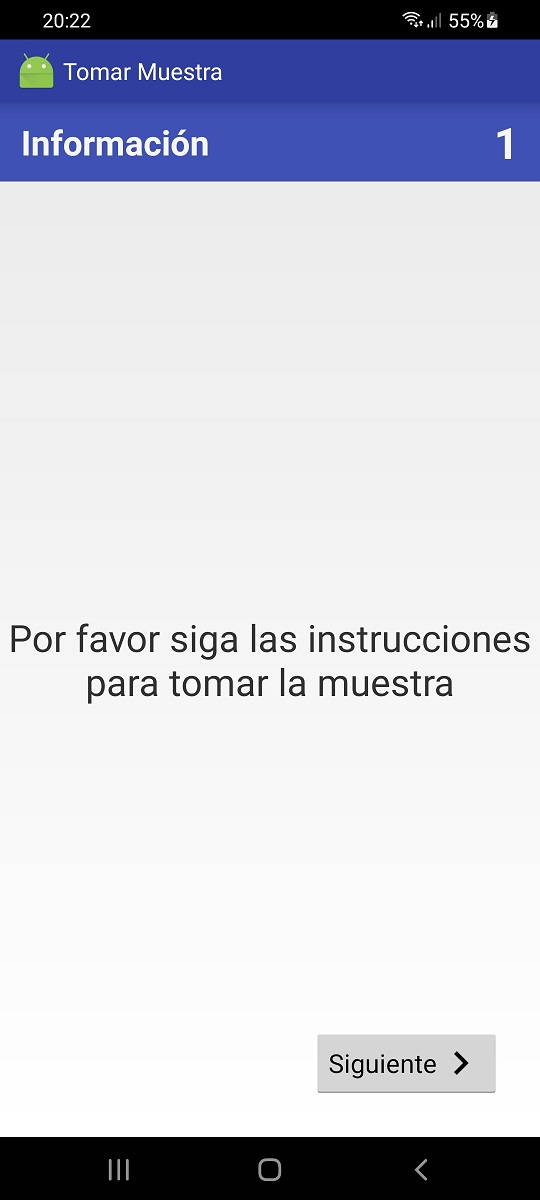
\includegraphics[scale=0.3]{50-anexos/C-steps/information_screen.jpg} 
    \caption{InformationStep en ejecución.}
\end{figure}


\subsection{InformationStepResult: El resultado de Mostrar información}
El resultado de mostrar información es nulo, es una clase vacía. Solo está para cerrar el circuito.





\section{SelectOneStep: Seleccionar una opción de un grupo de opciones}
SelectOneStep  se usa para solicitarle al científico ciudadano que seleccione una sola opción de varias opciones disponibles. Tiene un texto (title) que se muestran a modo de título o instrucciones. Las opciones disponibles para seleccionar son una lista de objetos SelectOneOption.
Cada objeto SelectOneOption tiene un id, textToShow y nextStepId, que se muestran en pantalla en forma de radio buttons.

Este caso particular de Step no tiene un identificador del siguiente Step a ejecutar (nextStepId), sino que cada opción seleccionable posee uno. Esto permite crear bifurcaciones en el Workflow, por ejemplo, se puede preguntar si se observa cierta característica y si la respuesta es si, pasar un PhotoStep para pedir que tome una foto de esa característica, pero si la respuesta es no, se puede saltar el paso de tomar una foto.

\begin{figure}[H]
  \centering
    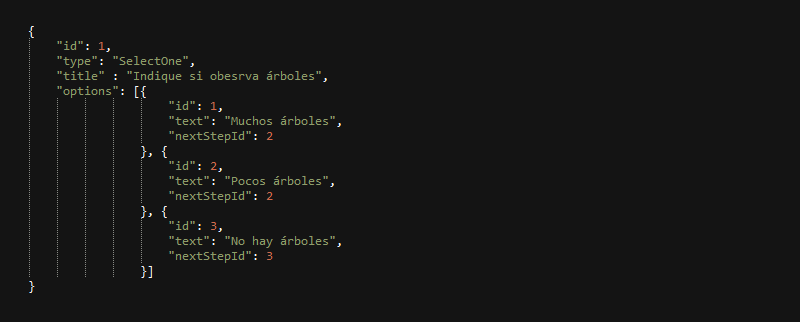
\includegraphics[scale=0.6]{50-anexos/C-steps/select_one_json.png} 
    \caption{SelectOneStep usando el generador de clases.}
\end{figure}	

\begin{figure}[H]
  \centering
    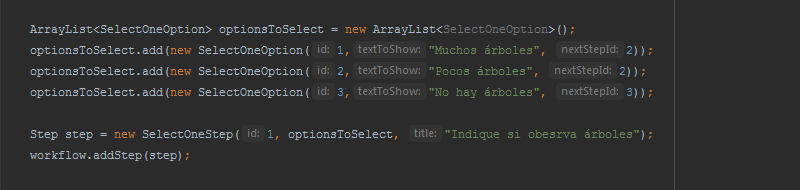
\includegraphics[scale=0.6]{50-anexos/C-steps/select_one_java.png} 
    \caption{SelectOneStep en Java.}
\end{figure}

\begin{figure}[H]
  \centering
    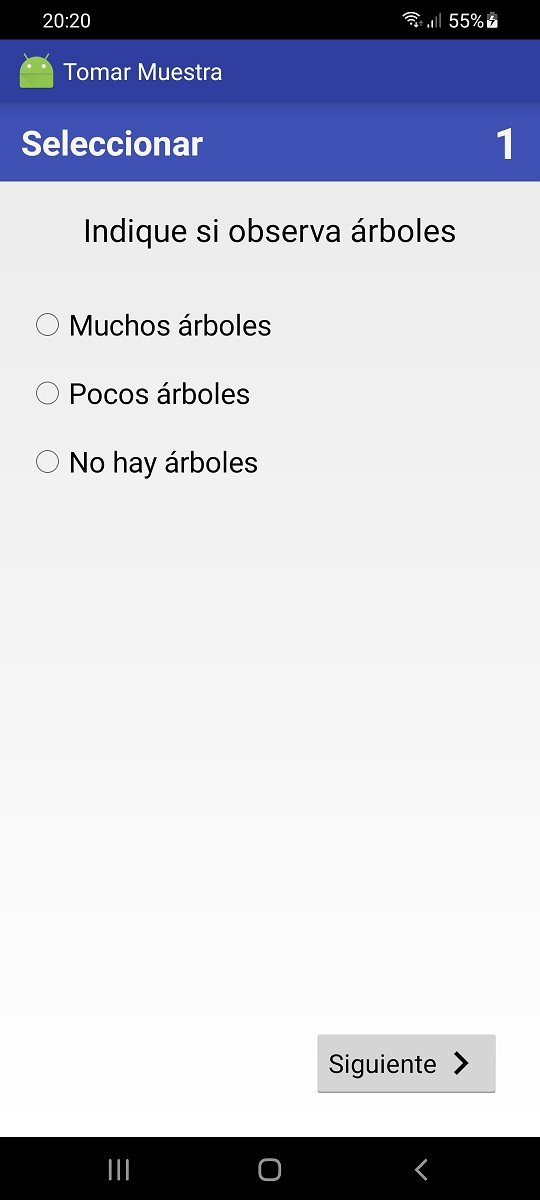
\includegraphics[scale=0.3]{50-anexos/C-steps/select_one_screen.jpg} 
    \caption{SelectOneStep en ejecución.}
\end{figure}


\subsection{SelectOneStepResult: El resultado de Seleccionar una opción de un grupo de opciones}
SelectOneStepResult contiene la opción seleccionada (un objeto SelectOneOption).





\section{MultipleSelectStep: Seleccionar varias opciones de un grupo de opciones}
MultipleSelectStep  se usa para solicitarle al científico ciudadano que seleccione una o más opciones de varias opciones disponibles. Tiene un texto (title) que se muestran a modo de título o instrucciones. Las opciones disponibles para seleccionar son una lista de objetos MultipleSelectOption.
Cada objeto MultipleSelectOption tiene un id, textToShow.
Las opciones disponibles para seleccionar se muestran en pantalla en forma de check-boxes.


\begin{figure}[H]
  \centering
    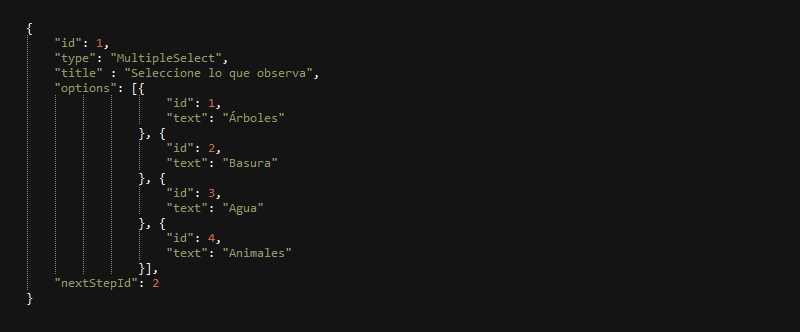
\includegraphics[scale=0.6]{50-anexos/C-steps/multiple_select_json.png} 
    \caption{MultipleSelectStep usando el generador de clases.}
\end{figure}	

\begin{figure}[H]
  \centering
    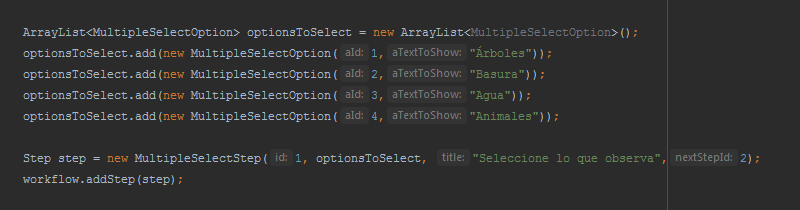
\includegraphics[scale=0.6]{50-anexos/C-steps/multiple_select_java.png} 
    \caption{MultipleSelectStep en Java.}
\end{figure}

\begin{figure}[H]
  \centering
    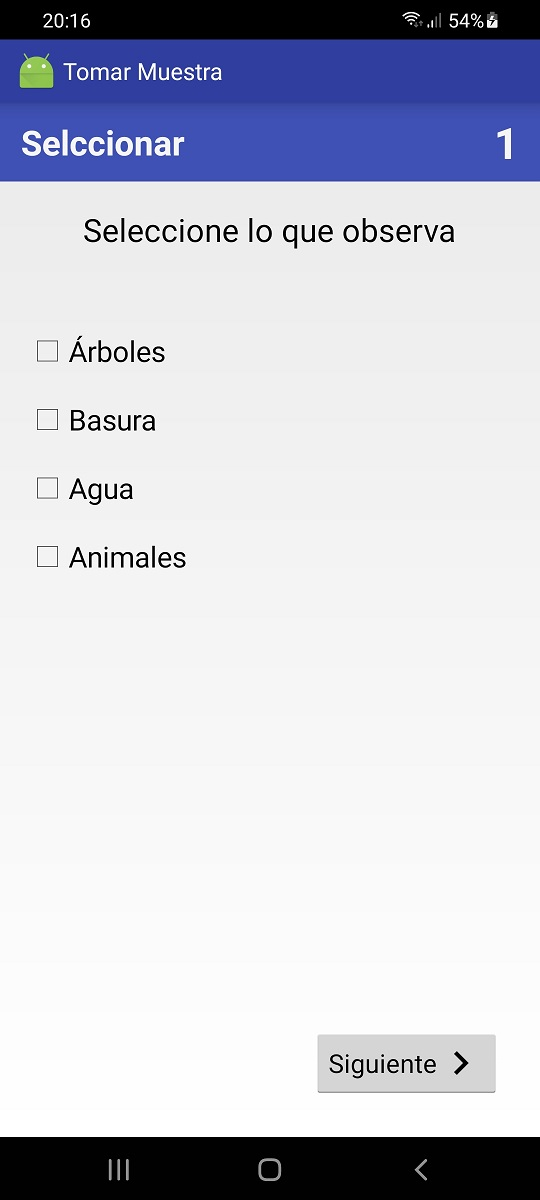
\includegraphics[scale=0.3]{50-anexos/C-steps/multiple_select_screen.jpg} 
    \caption{MultipleSelectStep en ejecución.}
\end{figure}


\subsection{MultipleSelectStepResult: El resultado de Seleccionar varias opciones de un grupo de opciones}
MultipleSelectStepResult contiene una lista de las opciones seleccionadas (una lista de objetos MultipleSelectOption).





\section{LocationStep: Posicionar la muestra en el mapa con el GPS}
LocationStep se usa para solicitarle al científico ciudadano que tome la posición con el GPS del dispositivo móvil. Tiene un texto (text) que se muestran a modo de instrucciones o mensaje. 

Permite usar el GPS o posicionar la muestra manualmente en el mapa.

\begin{figure}[H]
  \centering
    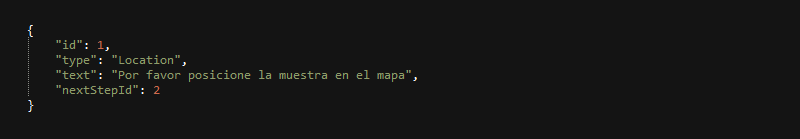
\includegraphics[scale=0.6]{50-anexos/C-steps/location_json.png} 
    \caption{LocationStep usando el generador de clases.}
\end{figure}	

\begin{figure}[H]
  \centering
    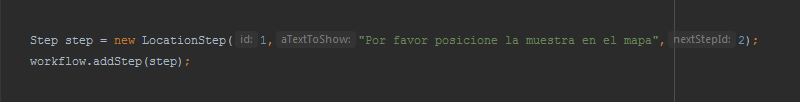
\includegraphics[scale=0.6]{50-anexos/C-steps/location_java.png} 
    \caption{LocationStep en Java.}
\end{figure}

\begin{figure}[H]
  \centering
    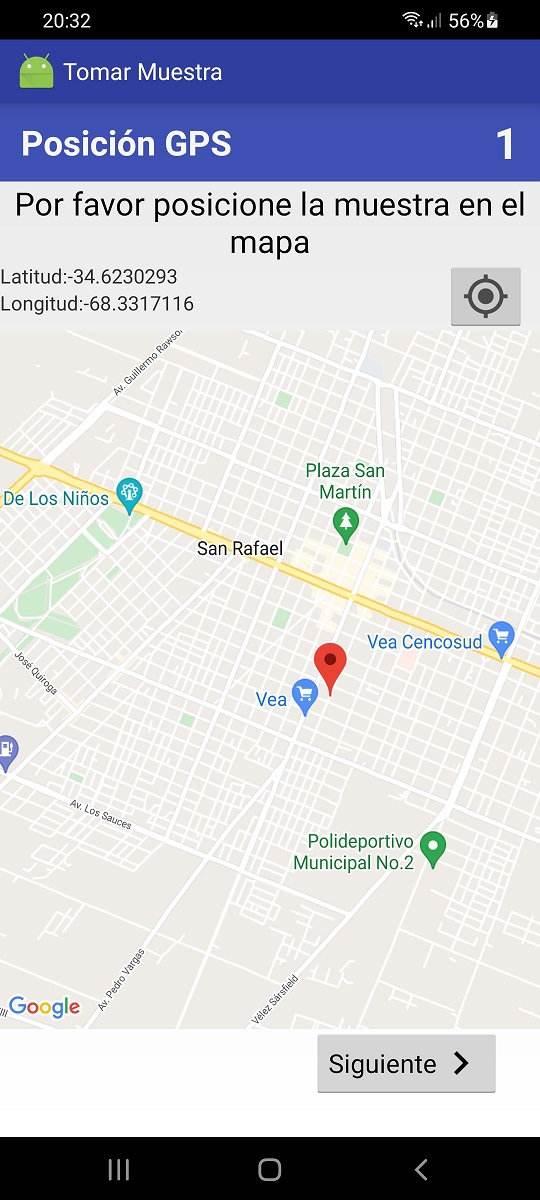
\includegraphics[scale=0.3]{50-anexos/C-steps/location_screen.jpg} 
    \caption{LocationStep en ejecución.}
\end{figure}

\subsection{LocationStepResult: El resultado de Posicionar la muestra en el mapa con el GPS}
LocationStepResult contiene la latitud y longitud (ambos de tipo double) de la posición GPS tomada.





\section{RouteStep: Grabar un recorrido en el mapa usando el GPS}
LocationStep se usa para solicitarle al científico ciudadano que grabe un recorrido con el GPS del dispositivo móvil. Tiene las siguientes propiedades:

\begin{itemize}
\item \textbf{text:} un texto que se muestran a modo de instrucciones o mensaje.
\item \textbf{interval:} [Opcional] el intervalo en milisegundos en el que se pedirán actualizaciones del GPS. Si no se especifica el valor por defecto es 5000.
\item \textbf{mapZoom:} [Opcional] el zoom con el que se muestra el mapa. Si no se especifica el valor por defecto es 15.
\end{itemize}


\begin{figure}[H]
  \centering
    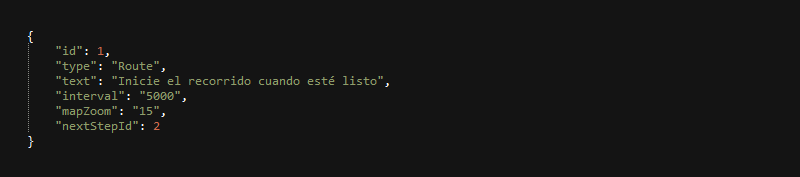
\includegraphics[scale=0.6]{50-anexos/C-steps/route_json.png} 
    \caption{RouteStep usando el generador de clases.}
\end{figure}	

\begin{figure}[H]
  \centering
    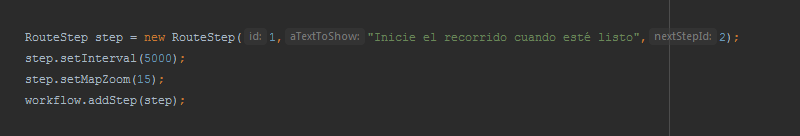
\includegraphics[scale=0.6]{50-anexos/C-steps/route_java.png} 
    \caption{RouteStep en Java.}
\end{figure}

\begin{figure}[H]
  \centering
    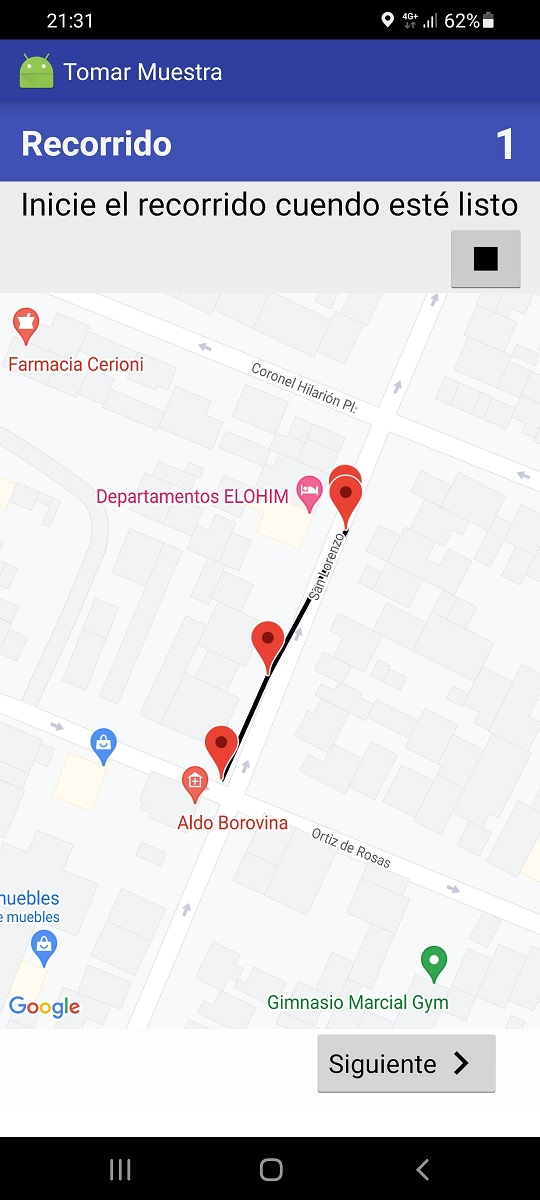
\includegraphics[scale=0.3]{50-anexos/C-steps/route_screen.jpg} 
    \caption{RouteStep en ejecución.}
\end{figure}


\subsection{RouteStepResult: El resultado de Grabar un recorrido en el mapa usando el GPS}
RouteStepResult tiene una lista de objetos de la clase Location proporcionada por Android.  Para
mas información sobre esta clase ver la documentación oficial de Android sobre Location \footnote{https://developer.android.com/reference/android/location/Location}.






\section{InsertTextStep: Ingresar texto}
InsertTextStep se usa para solicitarle al científico ciudadano que ingrese una anotación, que puede ser texto o números. Tiene las siguientes propiedades:

\begin{itemize}
\item \textbf{text:} un texto que se muestran a modo de instrucciones o mensaje.
\item \textbf{sampleText:} un texto, a modo de muestra.
\item \textbf{maxLength:} establece la cantidad máxima de caracteres permitidos.
\item \textbf{inputType:} indica el tipo de caracteres admitidos. Los valores pueden ser \textbf{text} para el ingreso de texto, \textbf{number} para el ingreso de número enteros, \textbf{decimal} para el ingreso de números con decimales.
\item \textbf{optional:} un booleano que indica si se puede dejar vacío (true) o si es obligatorio que ingrese una anotación (false).
\end{itemize}

\begin{figure}[H]
  \centering
    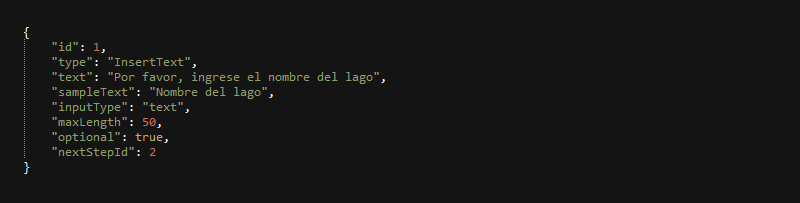
\includegraphics[scale=0.6]{50-anexos/C-steps/insert_text_json.png} 
    \caption{InsertTextStep usando el generador de clases.}
\end{figure}	

\begin{figure}[H]
  \centering
    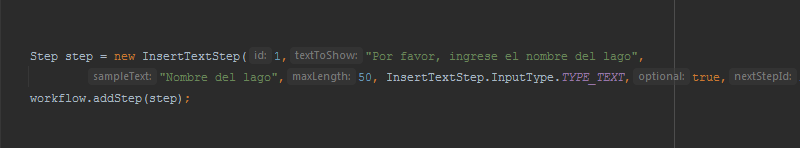
\includegraphics[scale=0.6]{50-anexos/C-steps/insert_text_java.png} 
    \caption{InsertTextStep en Java.}
\end{figure}

\begin{figure}[H]
  \centering
    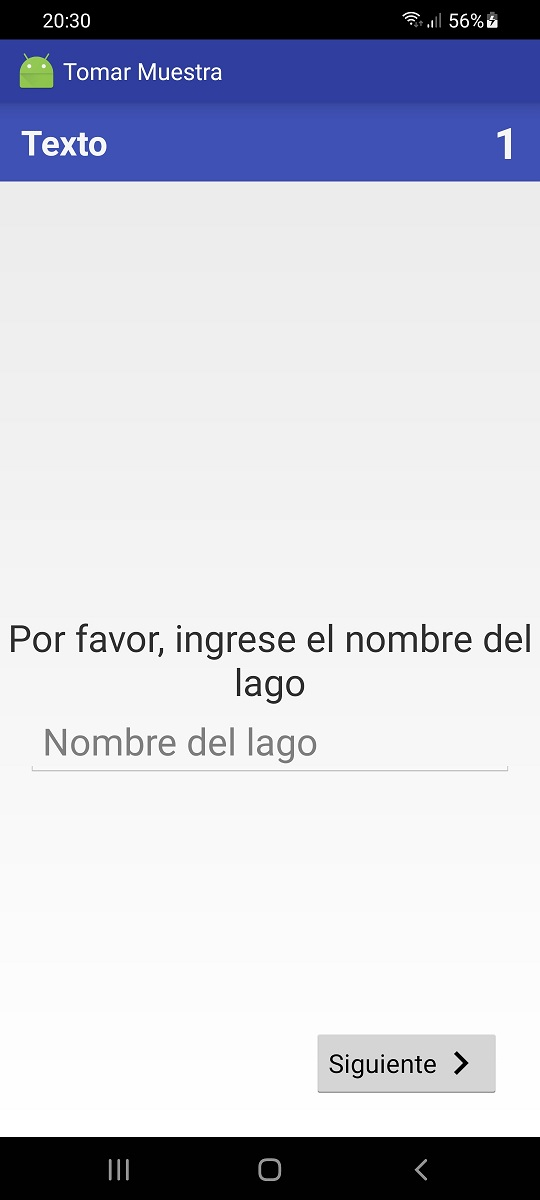
\includegraphics[scale=0.3]{50-anexos/C-steps/insert_text_screen.jpg} 
    \caption{InsertTextStep en ejecución.}
\end{figure}


\subsection{InsertTextStepResult: El resultado de Ingresar texto}
InsertTextStepResult contiene el String con la anotación ingresada.





\section{InsertDateStep e InsertTimeStep: Ingresar fecha y hora}
InsertDateStep e InsertTimeStep se usan para solicitarle al científico ciudadano que ingrese una fecha y una hora respectivamente. Tienen un texto que se muestran a modo de instrucciones o mensaje.


\begin{figure}[H]
  \centering
    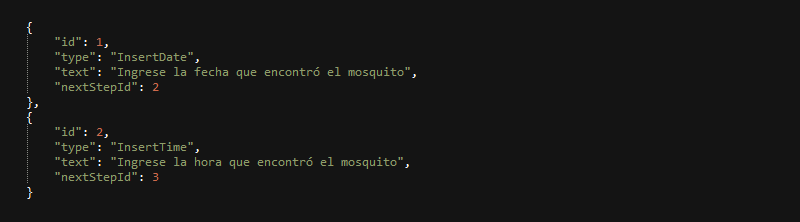
\includegraphics[scale=0.6]{50-anexos/C-steps/insert_date_time_json.png} 
    \caption{InsertDateStep e InsertTimeStep usando el generador de clases.}
\end{figure}	

\begin{figure}[H]
  \centering
    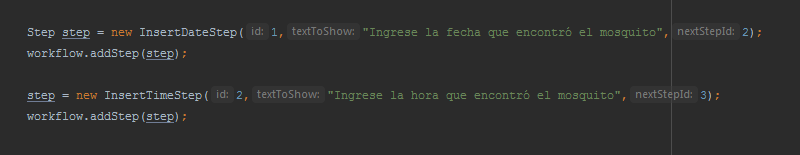
\includegraphics[scale=0.6]{50-anexos/C-steps/insert_date_time_java.png} 
    \caption{InsertDateStep e InsertTimeStep en Java.}
\end{figure}

\begin{figure}[H]
  \centering
    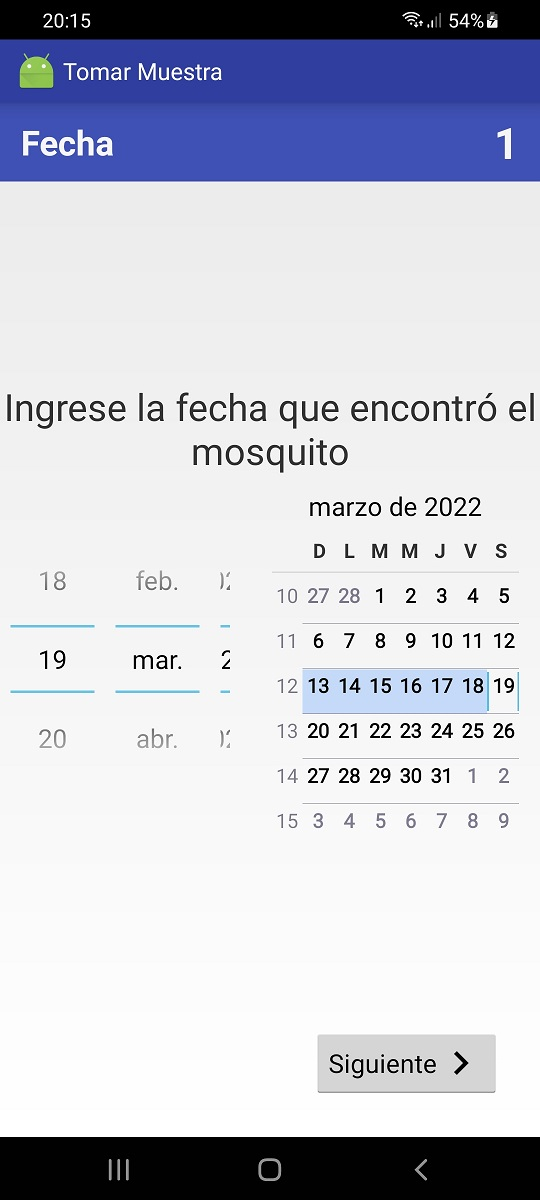
\includegraphics[scale=0.3]{50-anexos/C-steps/insert_date_screen.jpg} 
    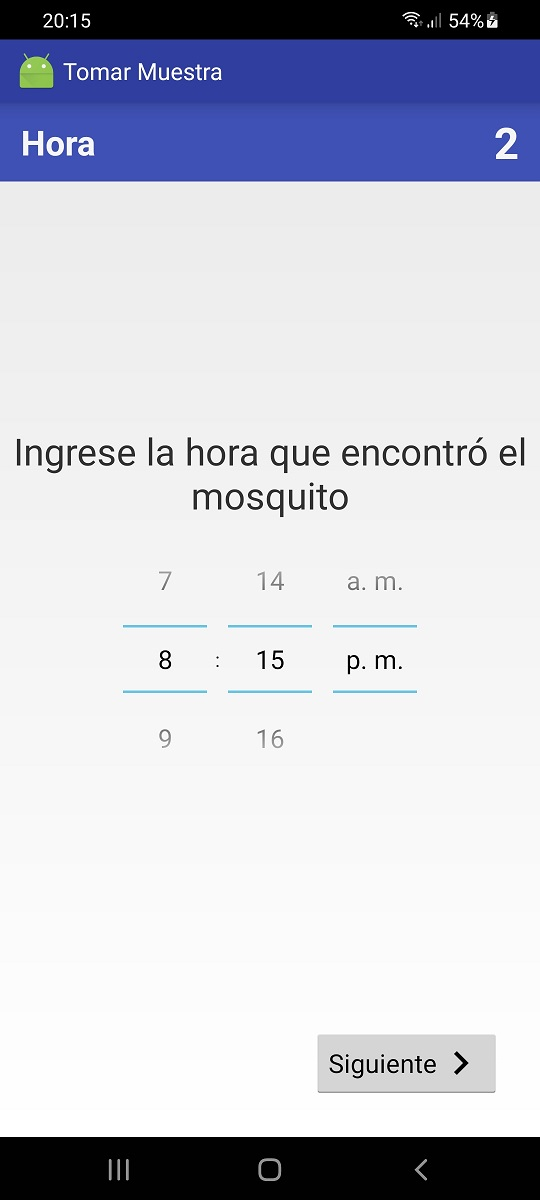
\includegraphics[scale=0.3]{50-anexos/C-steps/insert_time_screen.jpg} 
    \caption{InsertDateStep (izquierda) e InsertTimeStep (derecha) en ejecución.}
\end{figure}


\subsection{InsertDateStepResult e InsertTimeStep: El resultado de Ingresar fecha y hora}
InsertDateStepResult e InsertTimeStep tienen un objeto Date de Java que tiene la fecha o la hora según corresponda.






\section{Definir un nuevo Step, StepFragment y StepResult} \label{sec:definir_steps}
[TO-DO: acá vamos a explicar como definir un nuevo Step para extender el framework]



